\chapter{Study of Onion Data: Collection and Analysis}


\section{System}

For now, we are only working over onion data. We have three actors in model: Farmers who are producers of onion, traders who are collectively responsible for supply of onions across countries and consumers who purchase onions.

\begin{figure}[here]
\begin{center}	
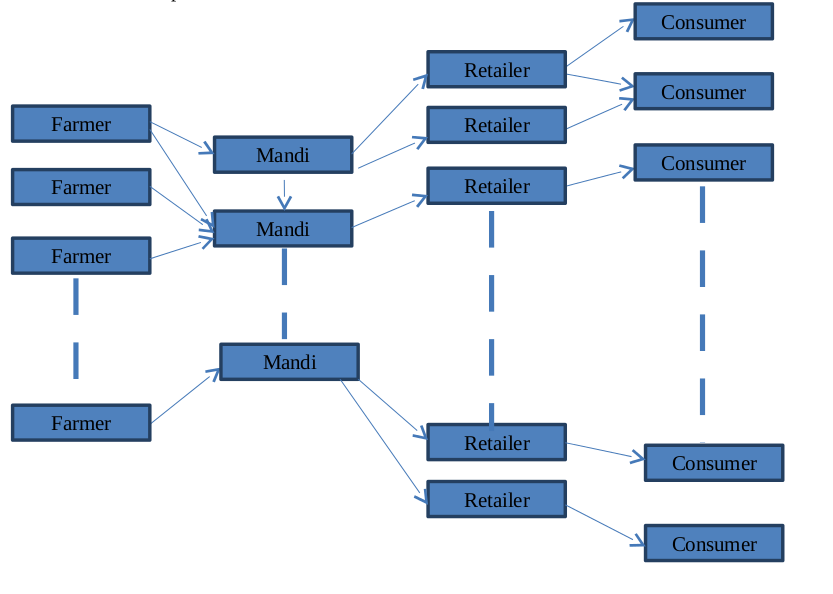
\includegraphics[scale=0.4]{3_1} 
\caption{Normal Supply Chain}
\label{fig:Normal Supply Chain}
\end{center}
\end{figure}

Farmers sell their produce to traders in nearest mandi offering better price. These traders sell these commodities to traders in other mandis or to retailers. Consumers purchase commodities for consumption from one of the retail stores. This way commodity reaches consumers from farmers following a huge chain of traders and retailers.

Under APMC act, mandis were established at different places across country so that farmers can sell their produce directly in mandi and get good returns (wholesale price). There are around 1500 mandis located in different places across country which log their daily arrival of onion, minimum, maximum, modal selling price per quintal of onion data to AGMARKNET. Retailers purchase from these mandis and sell to end customers at retail price. There are around 70+ centres across country which maintains retail price of onion on Ministry of consumer affairs website.

\section{Data we have}

We have following data:

\begin{enumerate}

\item Daily wholesale price of onion for 1514 mandis 
\item Daily arrival of onion information for 1514 mandis
\item Daily retail price of onion for 76 centres
\item Dates and location for hoarding reports from news articles
\item Longitude and latitude of mandis and centres

\end{enumerate}

Onion Data was collected from the the government websites,\cite{agmarknet} for arrival and wholesale price data and \cite{retailpricecollection} (Department of Consumer Affairs) for retail price data. Crawlers were written to collect the data from these datewise for the period of approximately 9.5 years, starting from Jan 2006 to Jun 2015. More data can be added simply by running crawlers again.


\section{Normal market behaviour}

\begin{enumerate}

\item Wholesale price is inversely proportional to arrival of commodity –higher production of crop will lead to more and more crop hitting market for sell. Hence more arrival which will result in surplus supply leading to drop in wholesale prices.

\item  Retail price is directly proportional to wholesale price – commodities reach customers through a long chain of traders and retailers, adding value at every stage of chain. So, retail price at which customers purchase commodities are more than wholesale.

\end{enumerate}

Any divergence from these characteristics of normal market leads to suspicious price hike situations/anomalies.


\section{What are the reasons for anomaly?}

Primarily there are 3 main reasons of anomaly.

\begin{enumerate}

\item \textbf{Government Policies:} When the price is low in the country, still government allows the export of onion in large amount, or supports it by keeping low minimum price then the prices can rise up drastically.

\item \textbf{Unseasonal Rainfall:} Due to insufficient rainfall, heavy rainfall or unseasonal rainfall, onion crop may get affected and the produce is low and wholesale price may rise up. But, this reason still is validating that wholesale price is inversely proportional to arrival, it may be just prices will be little higher than it was supposed to be.

\item \textbf{Hoarding:} When traders/wholesalers store the onion and does not release the stock in the market in the expectation of the good prices in the future, it will create the artificial deficit in the market and will shoot up the onion prices in the retail market due to low arrival in the retail market. The reason people do this is to expect the higher prices in the time of low production or may be for security. For example, if it is expected that this year the rainfall will be very low, then people may think that, due to that, production will be low in the future and so they will start storing onion right now and that will also create deficit in the market and price will go up. 

\end{enumerate}

So our study will focus on detection of anomalies in data and if possible comment on the possible reason for the anomaly.

\section{Mapping of wholesale price to retail price}

Voronoi Diagram is used to map every mandi to nearest possible centre. The centres with retail data were considered fixed points and country was divided into 76 regions. All the mandis falling in that region are mapped to the respective centre.


\begin{figure}[here]
\begin{center}	
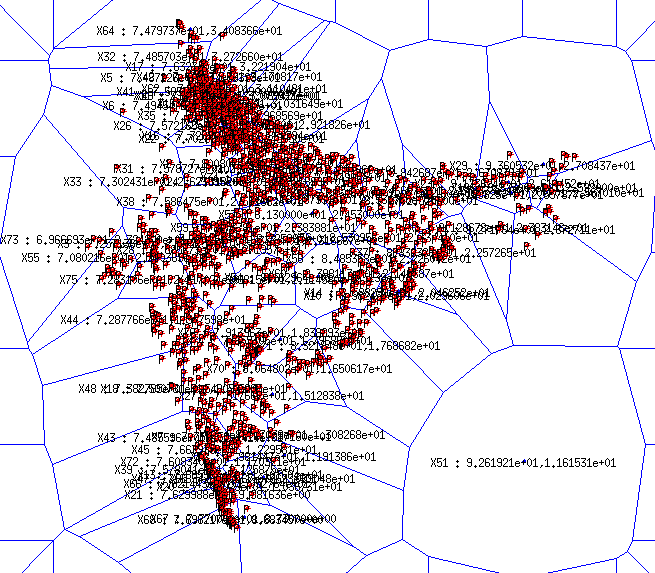
\includegraphics[scale=0.7]{3_2} 
\caption{Voronoi Diagram}
\label{fig:Voronoi Diagram}
\end{center}
\end{figure}


After all the mandis are mapped to their nearest centre, wholesale and arrival at every centre is computed. Wholesale price at centre is average of modal price of all mandis in its region and arrival was computed as the sum of the arrival at the mandis in its region. While calculating the wholesale price, the distance between centre and the mandi was not considered.

Corresponding to every date and location of hoarding news report, values like current year arrival, last year arrival, Percentage difference in wholesale- retail etc. were computed. Following table resulted from these computations.


\section{How to Define Anomaly?}

To answer this question, we went through the series of the news articles when the hoarding is in the news. Then looking over those articles, we try to see that why they are reporting to news, what happened so that people are giving it name of hoarding and how reporters are making conclusion that it may be the class of the hoarding.

